
\chapter{Budowa sprzętowego generatora liczb losowych}
\section{Projektowanie robota}
\subsection{Prototypowanie}

Przy całym procesie budowy robota wykorzystano technologię druku 3D. Pozwala na szybkie modyfikacje przy 
jednoczesnym zachowaniu bardzo wysokiej dokładności i jakości wykonania elementów. Dzięki temu podczas budowy prototypów a 
pózniej ostatecznej wersji robota można było w prosty sposób modyfikować, projektować i zmieniać każdy element składowy 
robota. Pomimo tego, że proces druku 3D w szczególności dużych skomplikowanych elementów jest stosunkowo czasochłonny to jest to
najlepsza dostępna nam technologia do wykorzystania w tego rodzaju projektach.

Głównym założeniem podczas projektowania i budowy robota było założenie modułowości. Oznacza to, że każdy element jest wymienny i łatwo dostępny.
Dzięki takiemu podejściu wymienianie elementów w przypadku awarii czy też małe modyfikacje wynikające z udoskonalania działania robota
są znacząco prostsze i przede wszystkim szybsze niż gdyby cały robot był jednolitą bryłą.

Proces projektowania robota rozpoczęto od przeanalizowania różnych metod wykonywania rzutu kością.
Po przeanalizowaniu kilku pomysłów, zdecydowano się na rozwiązanie wykorzystujące obrotowy 
kubek, wewnątrz którego kość porusza się i odbija od ścianek. Wariant ten roboczo nazwano betoniarką od podobnej 
zasady działania. Taki mechanizm zapewnia rzut zbliżony do takiego wykonanego przez człowieka, a 
jednocześnie jest prosty w konstrukcji. Obracający się kubek został 
zaprojektowany tak, aby jego prędkość obrotową i czas trwania obrotu można było w prosty sposób kontrolować poprzez kod napisany w Pythonie.
W celach testowych został skonstruowany prototypowy model robota.

Pierwszy prototyp robota składał się z metalowych prętów służących za stelaż oraz elementów wydrukowanych na drukarce 3D.
Tymi elementami były: kubek, ramię służące do montażu kubka, uchwyty do prętów oraz płytka mocująca do kamery. Dodatkowo
wykorzystano silnik prądu stałego napędzający kubek oraz sterownik służący do zasilania i sterowania ruchem silnika.

\begin{figure}[H]
    \centering
    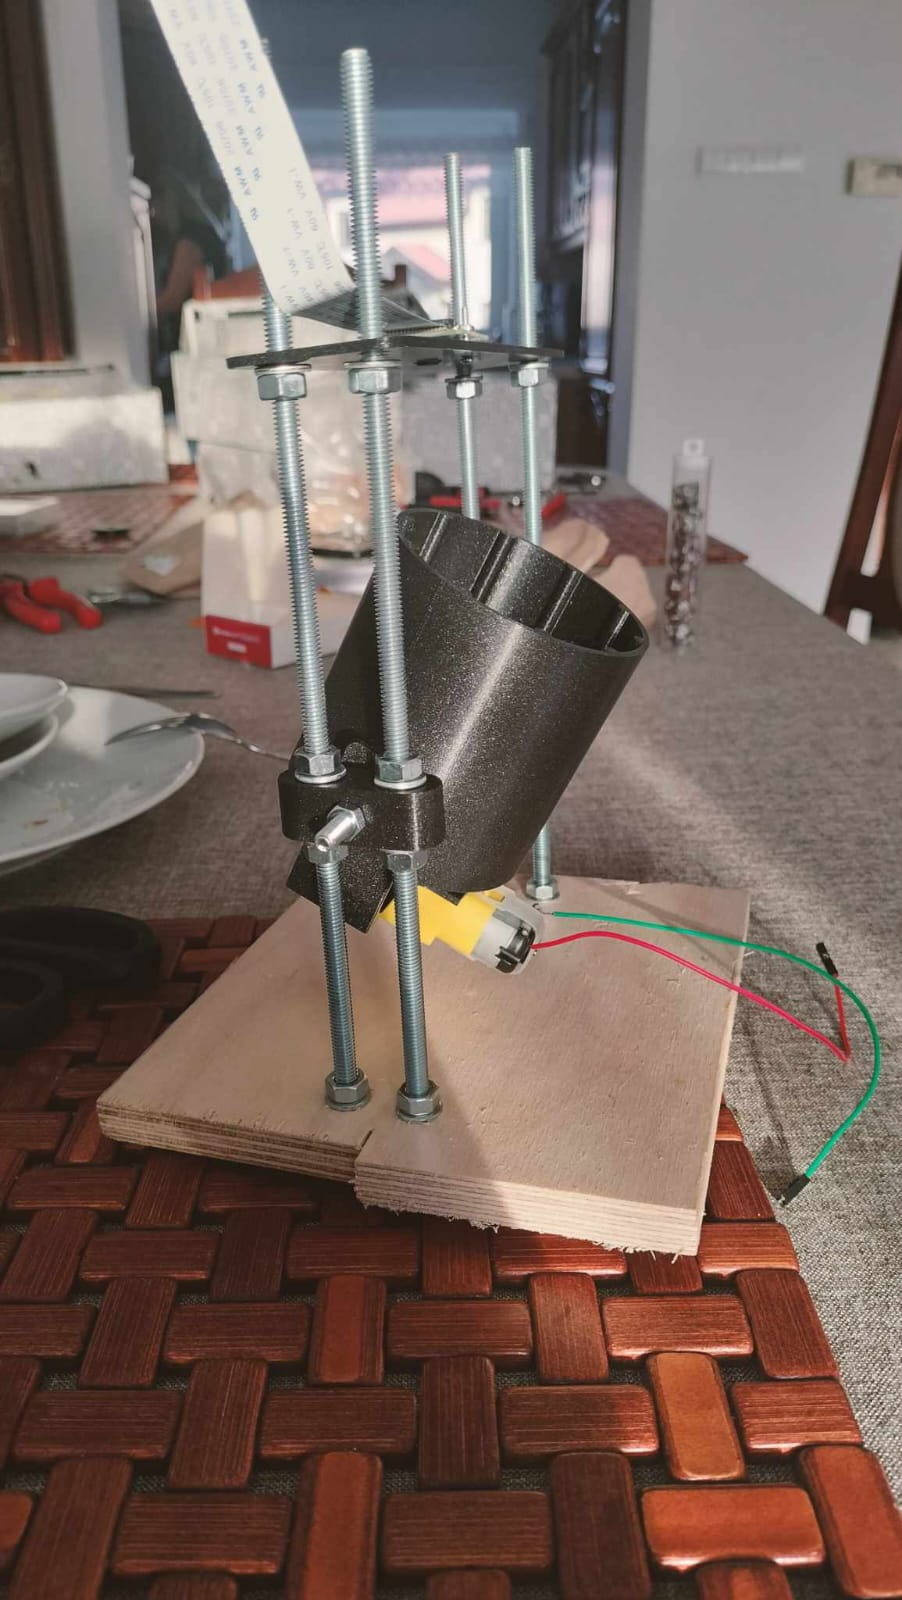
\includegraphics[width=0.25\linewidth, trim={35mm 75mm 35mm 30mm}, clip]{chapters/03-praca-wlasna/figures/pierwszy}
    \caption{\label{fig:pierwszy}Pierwszy prototyp}
\end{figure}

Do pierwszych testów robota zaprojektowano kilka wariantów kształtów kubków. Przy ich projektowaniu wymiary wzorowano na dostępnych tradycyjnych kubkach do gry w kości.
Przyjęto, że odpowiedni do tego zadania kubek powinien
zawierać pewnego rodzaju nieróności na ściankach. Dzięki temu kostka nie będzie się ślizgać po ściance a zacznie się odbijać od tych nierówności, co 
będzie lepiej imitowało rzut kością wykonany przez człowieka. Z tego powodu z założenia odrzucono tradycyjny model kubka do gry w cylindrycznym kształcie 
o gładkich ściankach. Zaprojektowano cztery wersje kubka, które następnie przetestowano umieszczając w środku kość do gry i obracając kubek wokół osi przechodzącej przez środek kubka.
Najlepszym wariantem okazał się być cylindryczny kubek z dodatkowymi pionowymi żebrami (numer 3 na poniższym zdjęciu), o które kostka się odbijała podczas kręcenia. Jego główną zaletą
nad resztą testowanych kubków był fakt, że nie posiada on narożników, w których kość, trafiając podczas obracania kubkiem, mogła utknąć dociskana przez 
siłę odśrodkową.

\begin{figure}[H]
    \centering
    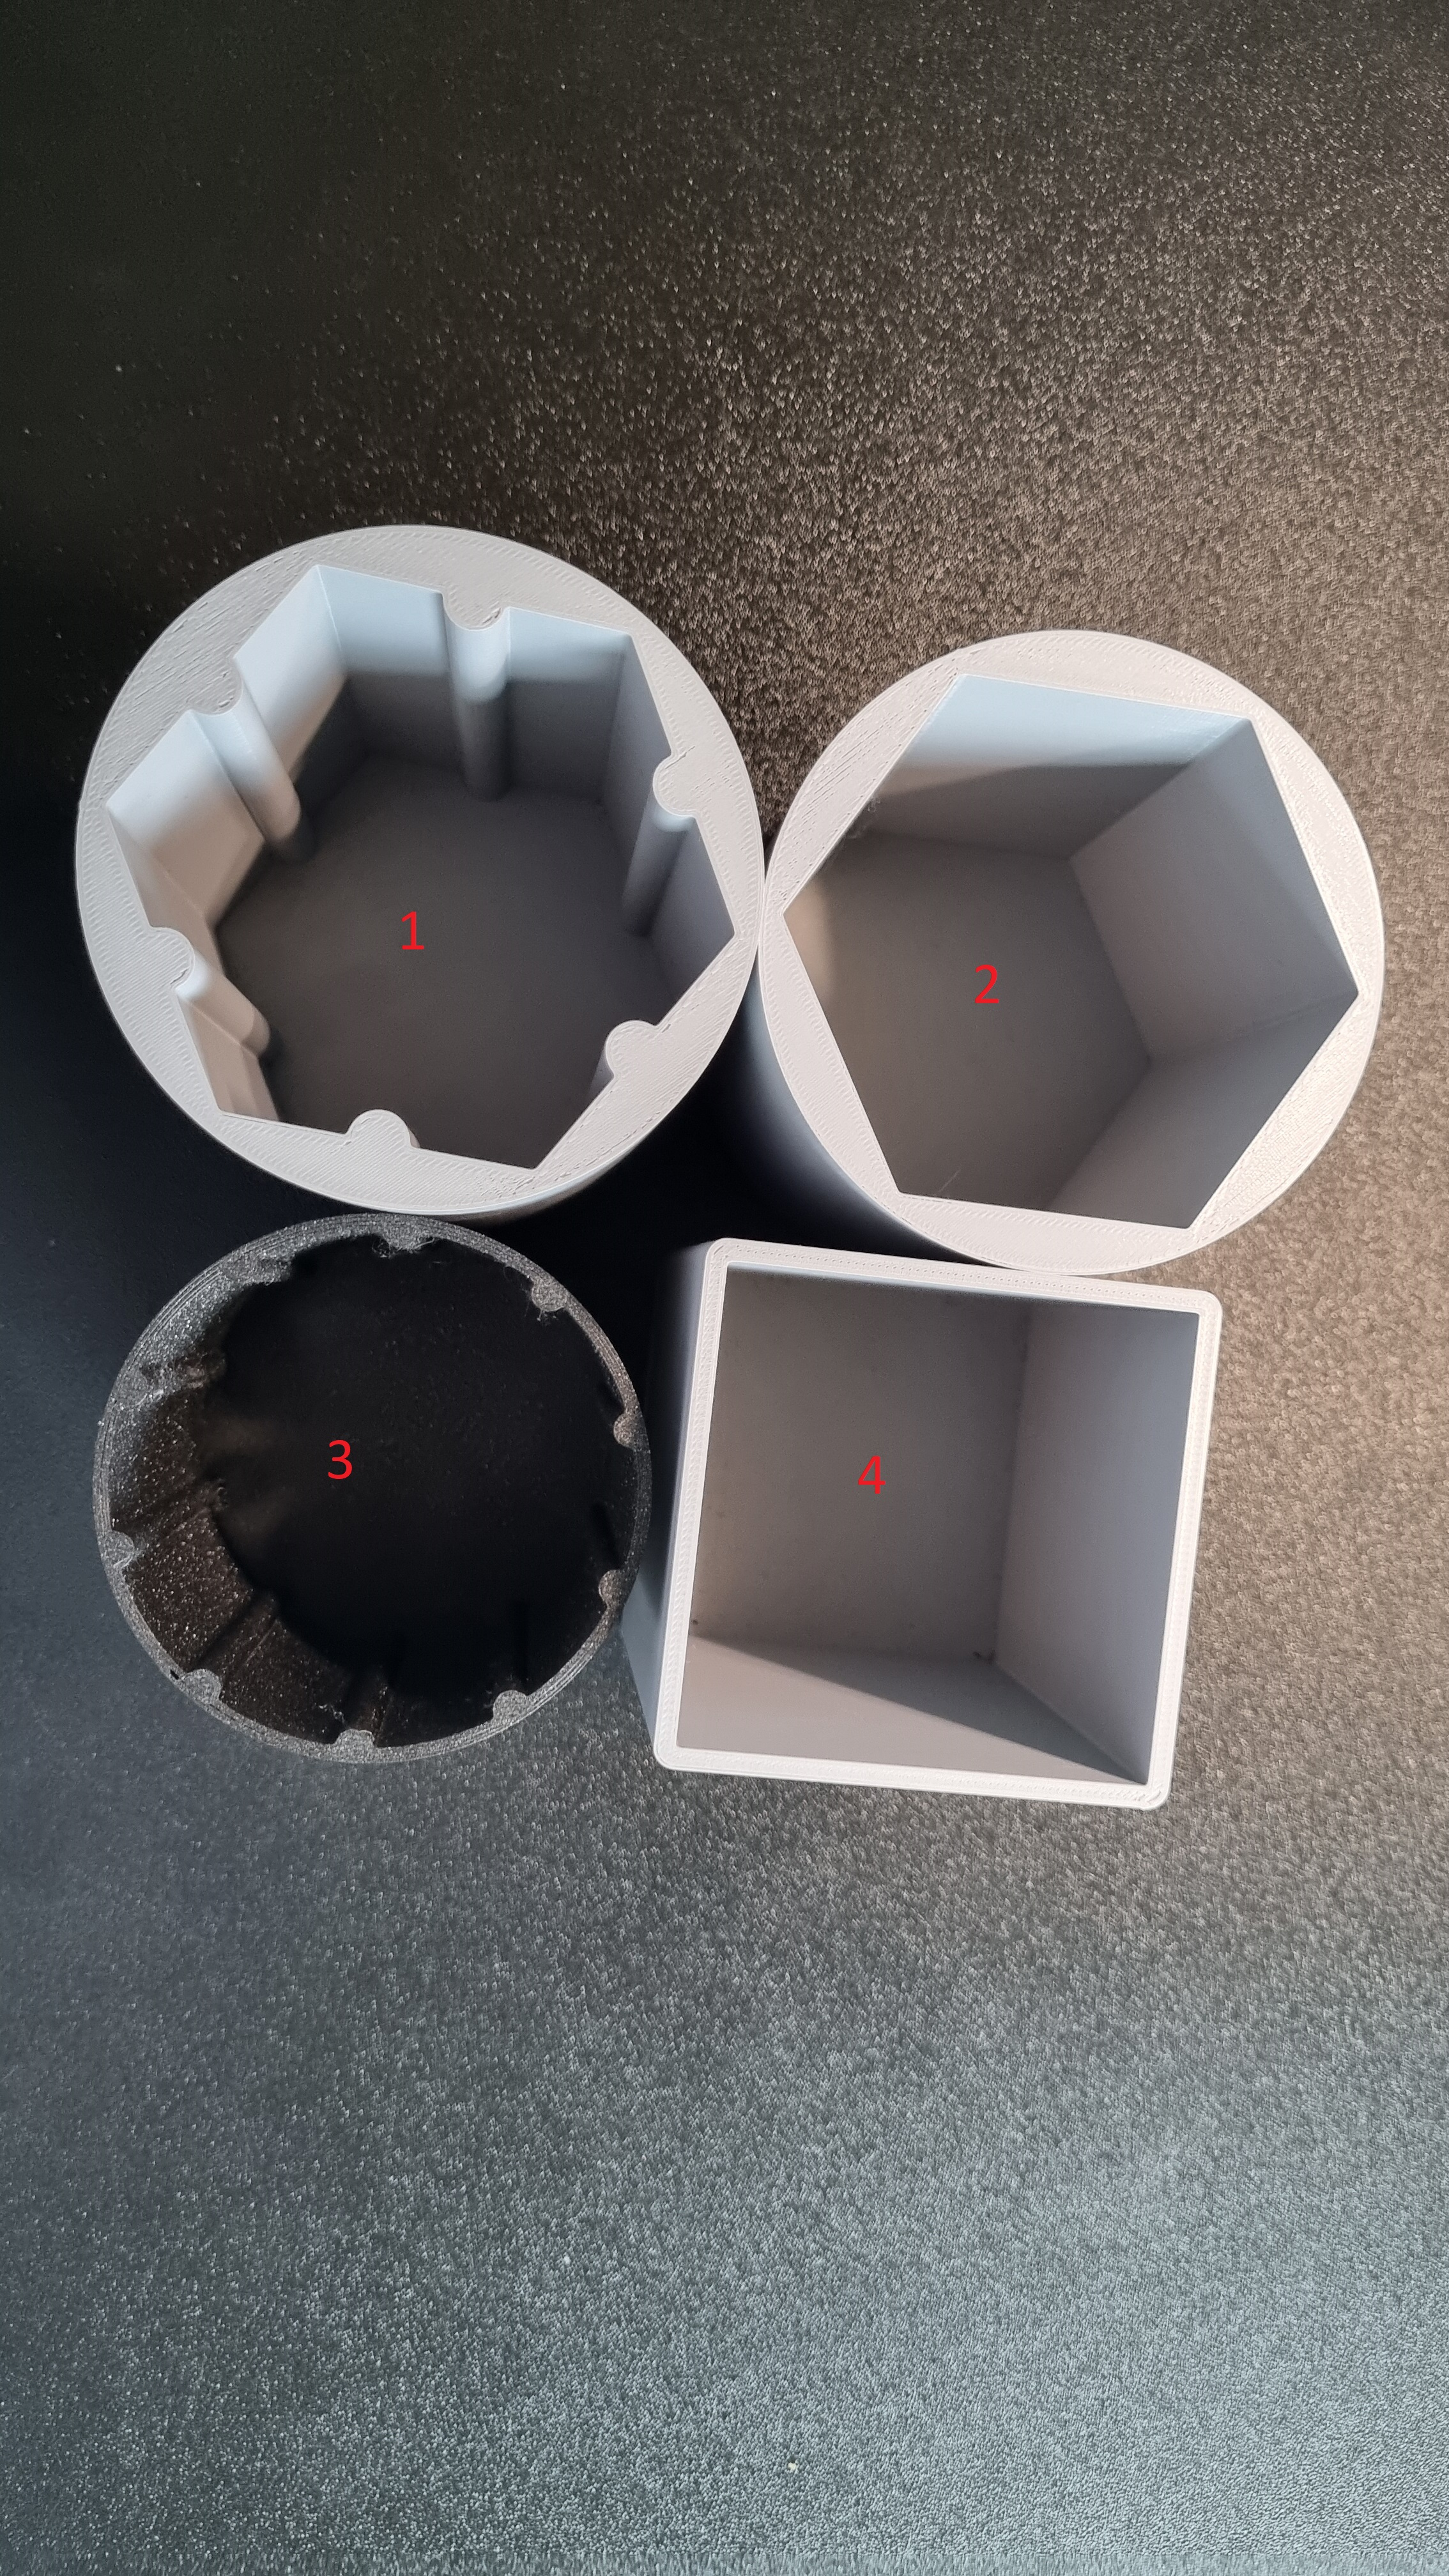
\includegraphics[width=0.65\linewidth, trim={35mm 380mm 20mm 240mm}, clip]{chapters/03-praca-wlasna/figures/kubki.jpg}
    \caption{\label{fig:kubki}Testowane warianty kubków}
\end{figure}

W trakcie poszukiwania literatury w temacie rzutów kością natrafiono na artykuł opisujący eksperyment, który wykorzystywał bardzo podobne urządzenie.
Urządzenie opisano w następujący sposób: \textit{For the machine-throwing, we used a newly constructed, electrically-driven machine which had a rectangular 
cage, 25 inches in length and four by four inches at the ends, made of quarter-inch wire mesh. This cage rotated on an axis through the middle, throwing the dice
from one end to the other over a rough course which made them bound about considerably.}\cite{PK}

Po pierwszych testach okazało się, że niezbędny do uzyskania zamierzonego efektu będzie mechanizm, który będzie 
wychylał cały kubek wraz z silnikiem, który odpowiada za jego obrót. Z początku planowano wykorzystanie
serwomechanizmu jednak to rozwiązanie odrzucono, ponieważ większość dostępnych serwomechanizmów, ma
ograniczony obrót do $180^{\circ}$ lub $360^{\circ}$ a to limitowałoby możliwości mechanizmu służącego do wychylania kubka.
Ostatecznie w tym celu wybrano mały silnik krokowy momentem obrotowym 34.3 mN.m, który jest wystarczający do wychylania kubka. 
Silnik ten obraca układem dwóch kół zębatych przedstawionych na zdjęciu poniżej.

\begin{figure}[H]
    \centering
    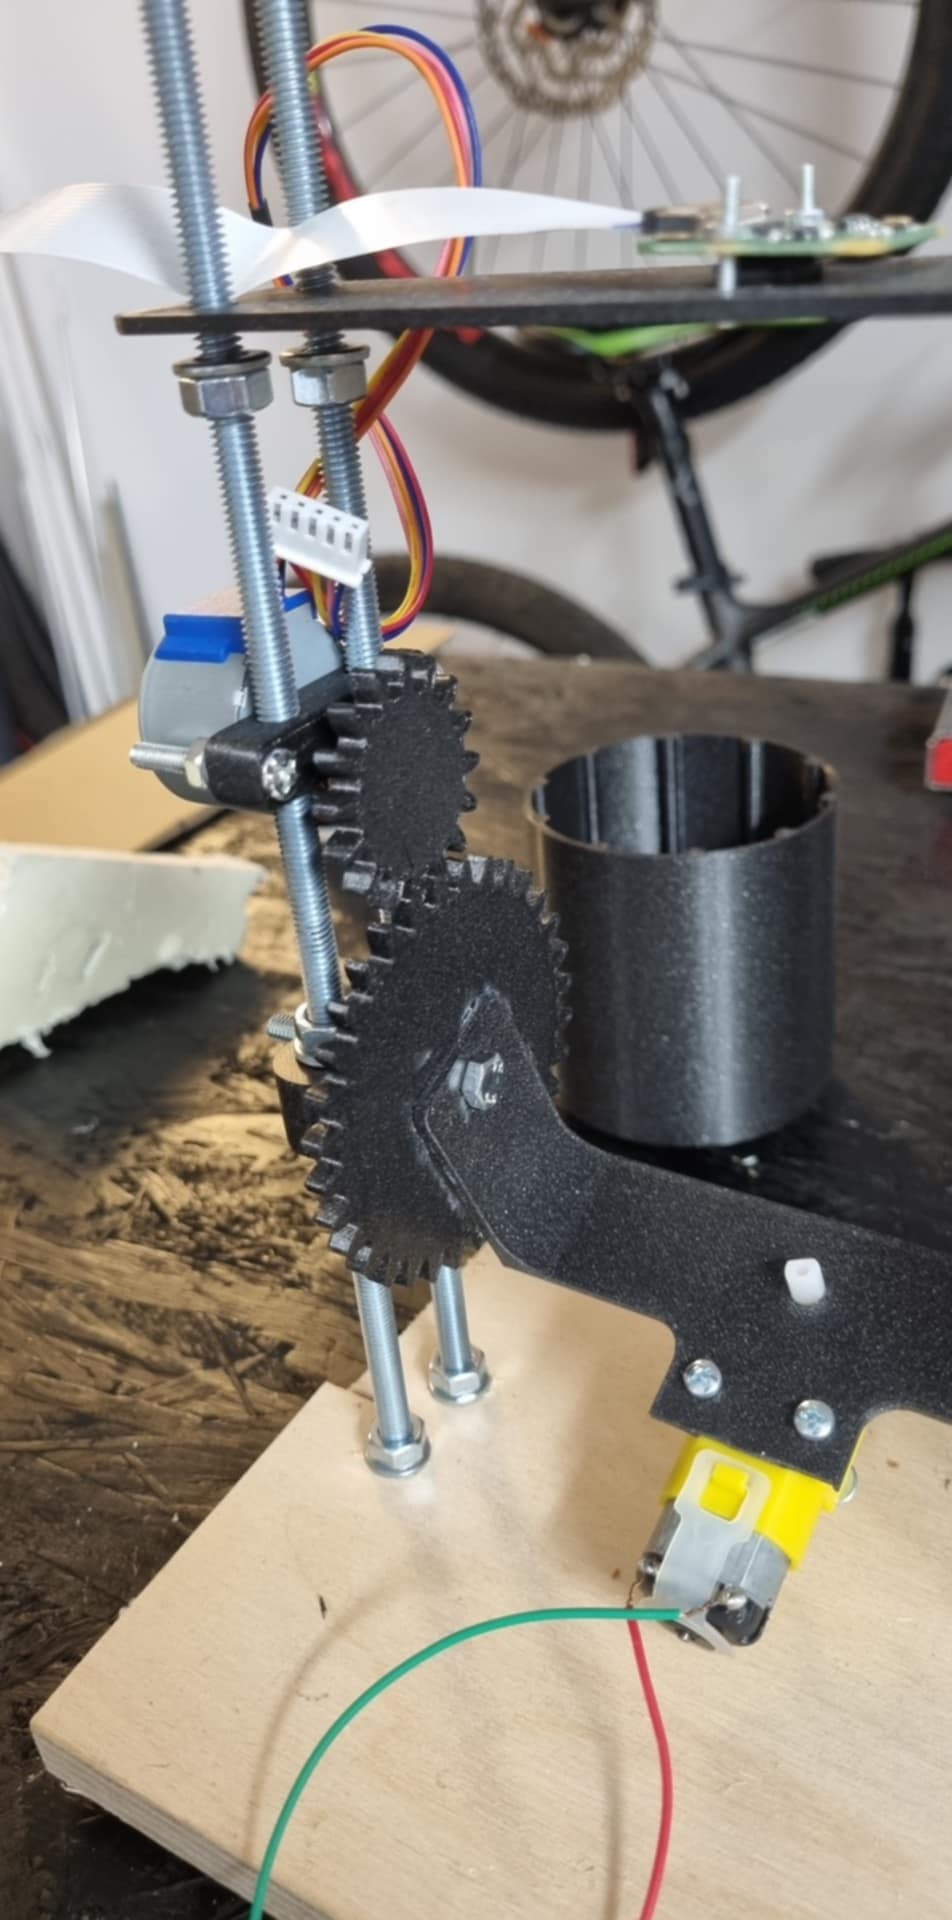
\includegraphics[width=0.25\linewidth, trim={65mm 75mm 0mm 180mm}, clip]{chapters/03-praca-wlasna/figures/koła_zębowe.png}
    \caption{\label{fig:zebatki}Koła zębate}
\end{figure}

Podczas testów pierwszej wersji robota wykorzytującej obrotowy kubek powstał pomysł alternatywnego rozwiązania.
Rozwiązanie to implementuje inne podejście do rzutu kością. Zamiast obracać cały kubek, a dodatkowo wychylać go,
wykorzystany został trwale zamontowany kubek, na którego dnie znajduje się śmigło, które podcina leżącą na dnie kość.
Takie rozwiązanie znacząco upraszcza cały mechanizm robota oraz bardzo przyspiesza proces losowania liczby. Ten wariant 
nazwano roboczo blenderem, również od podobnej zasady działania mechanizmu.

Przy projektowaniu drugiego wariantu robota został wykorzystany ten sam stelaż złożony z metalowych prętów co w 
pierwszym wariancie. Na drukarce 3D wydrukowano dodatkowe części, niezbędne do realizacji tego wariantu.
Zaprojektowano i wydrukowano nowy kubek, śmigło oraz mocowanie dla silnika. Kubek został przystosowany do montażu 
silnika prądu stałego oraz śmigła.

W trakcie testów zauważono, że procesor robota nagrzewa się do wysokich temperatur podczas intensywnej pracy, 
co mogło negatywnie wpływać na jego wydajność i żywotność. Aby temu zapobiec, w projekcie zdecydowano się na 
zastosowanie radiatorów, które miały pomóc w rozproszeniu nadmiaru ciepła, oraz wentylatora, który 
wspomagał cyrkulację powietrza wokół procesora. Dzięki temu rozwiązaniu udało się obniżyć temperaturę pracy 
procesora, która teraz utrzymuje się w granicach $55^{\circ}$C w czasie rzutów i spada po ich zakończeniu do około $45^{\circ}$C,
co zapewnia stabilne i bezpieczne działanie całego systemu. 

\begin{figure}[H]
    \centering
    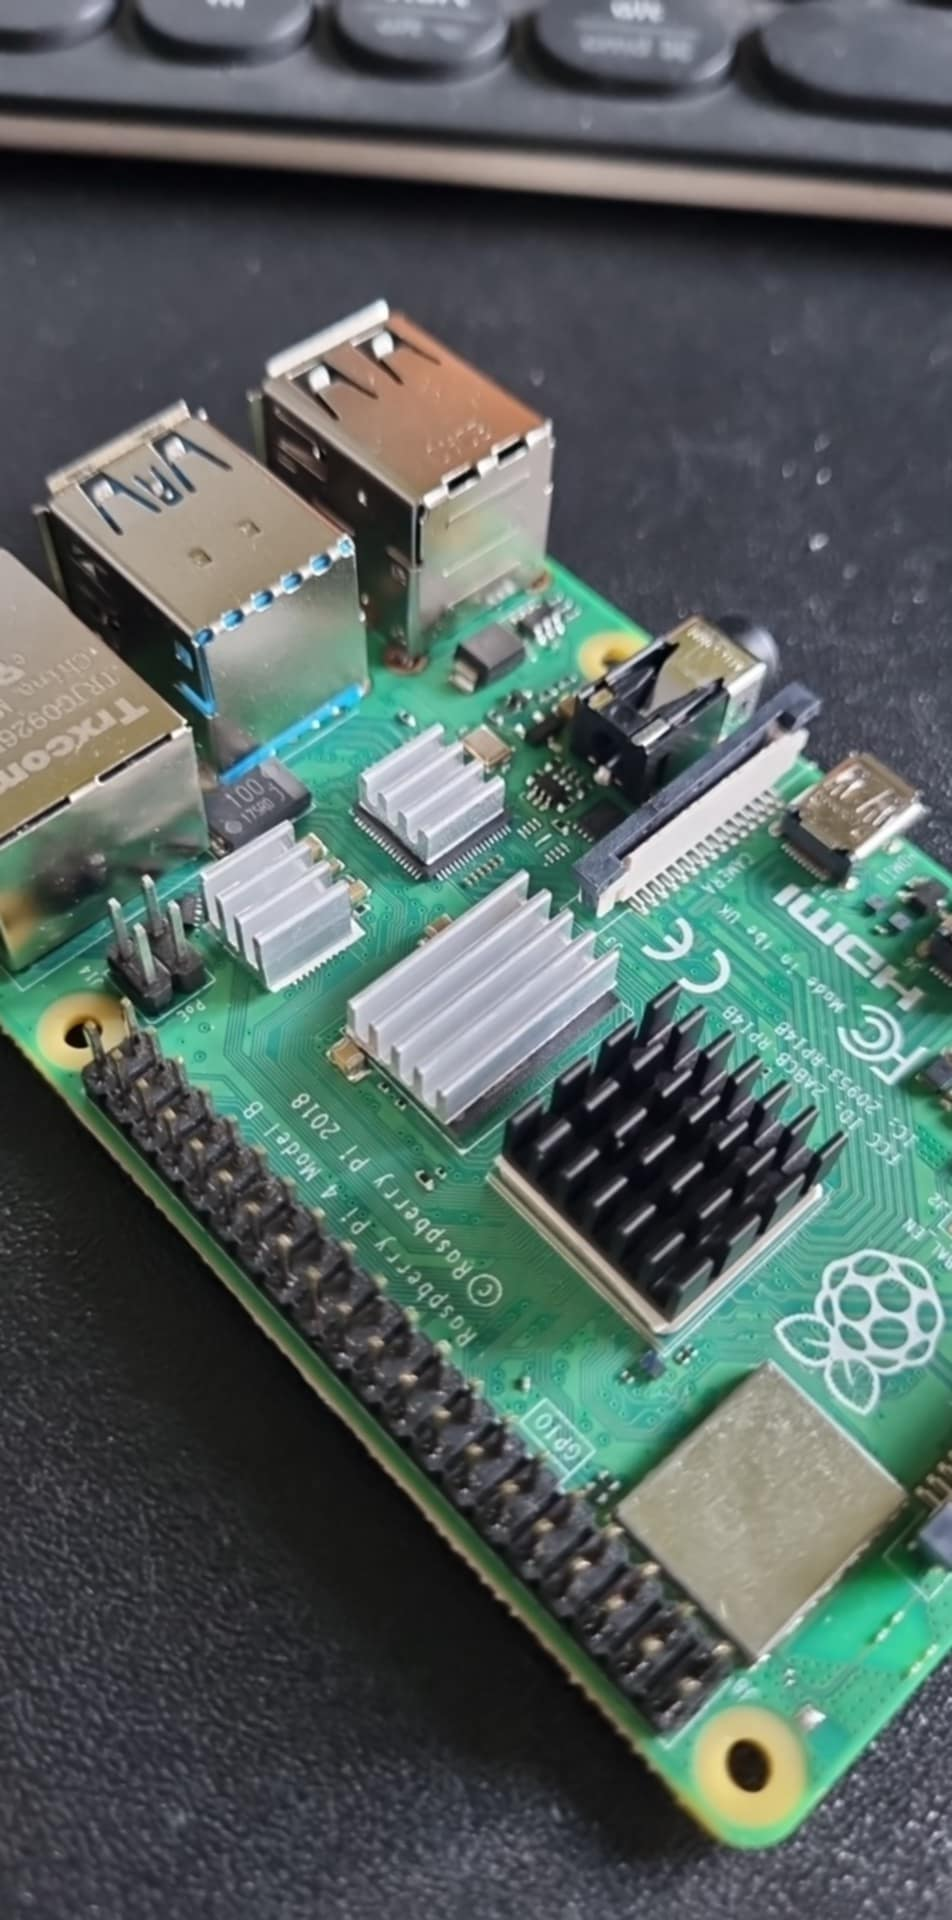
\includegraphics[width=0.25\linewidth, trim={0mm 50mm 0mm 120mm}, clip]{chapters/03-praca-wlasna/figures/now_we_are_cool.png}
    \caption{\label{fig:zimno}Dodane radiatory}
\end{figure}

Duże znaczenie ma również wykorzystywana kość. Od jej koloru i tekstury zależy jakość zdjęć zrobionych przez
zamonotowaną kamerę. Poniżej przedstawiono dwa przykłady zdjęć i różnic w ich czytelności zależnych od koloru kości.

\begin{figure}[H]
    \centering
    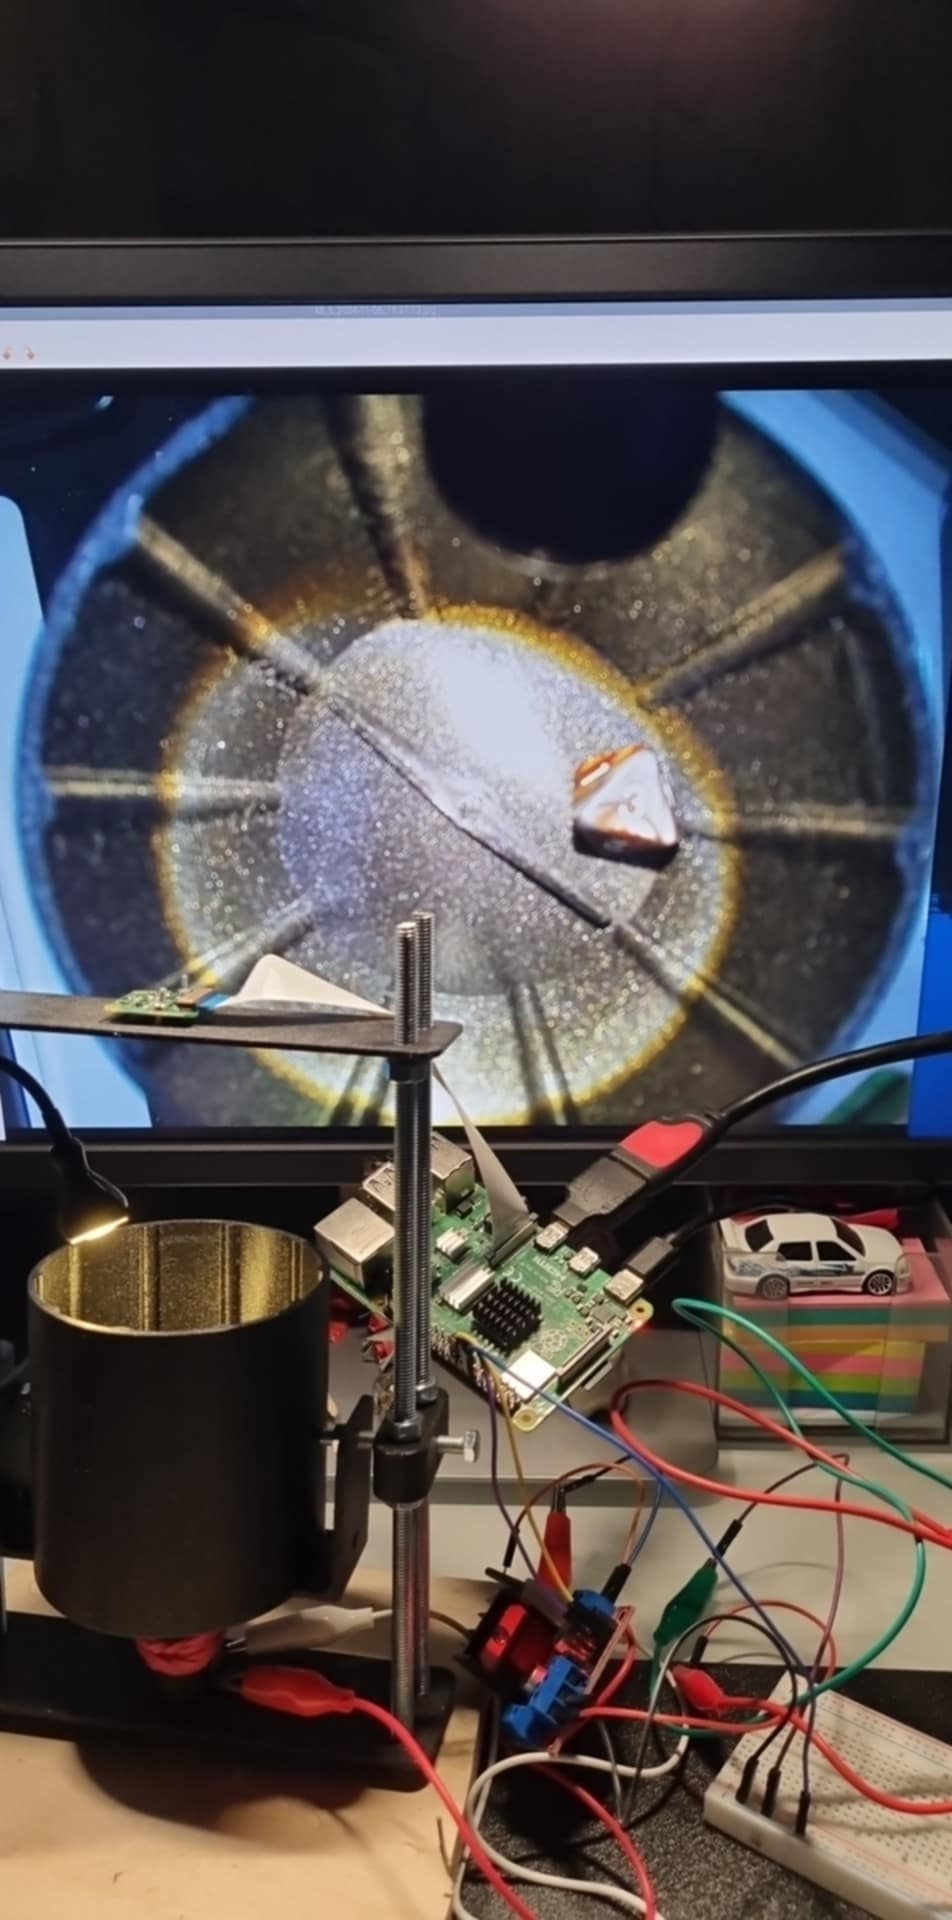
\includegraphics[width=0.25\linewidth, trim={0mm 30mm 0mm 120mm}, clip]{chapters/03-praca-wlasna/figures/nie_widac.png}
    \caption{\label{fig:nie_widac}Kość z teksturą}
\end{figure}

\begin{figure}[H]
    \centering
    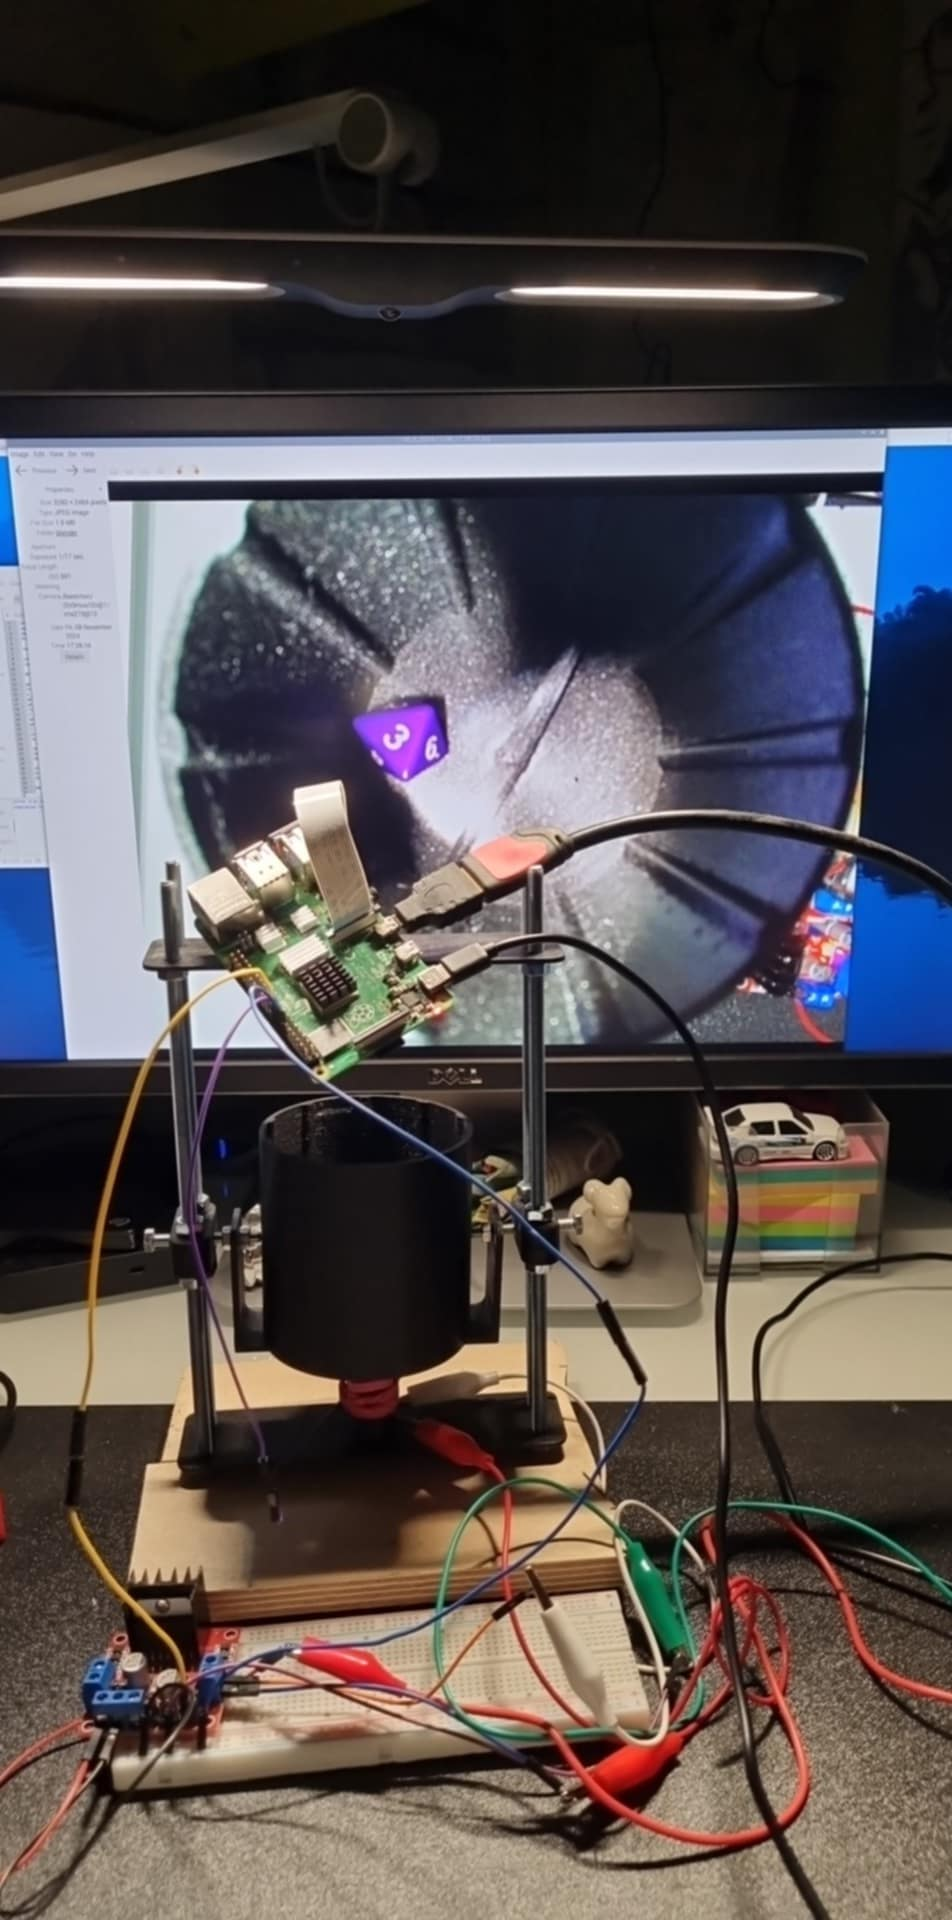
\includegraphics[width=0.25\linewidth, trim={0mm 30mm 0mm 120mm}, clip]{chapters/03-praca-wlasna/figures/widac.png}
    \caption{\label{fig:widac}Jednobarwna kość}
\end{figure}


W obu wariantach dużym problemem był złej jakości obraz z kamery. W tym celu zaprojektowano system oświetlenia składający się z diod
LED sterowanych przy pomocy układu ULN2803A. Dzięki temu wnętrze kubka stało się dużo jaśniejsze co pozwala kamerze na
robienie zdjęć lepszej jakości. Dodatkowo rozświetlenie wnętrza kubka na tyle poprawiło
jakość zdjęć, że pozwoliło to na obniżenie kamery względem kubka. Spowodowało to że wysokość prototypu zmniejszyła się o około 5cm - 
co było znaczącą poprawą, ponieważ jednym z założeń postawionych na początku budowy było stworzenie urządzenia o niewielkich rozmiarach.
Dzięki tym zabiegom otrzymywane zdjęcia stały się dużo bardziej wyraźne oraz pole widzenia kamery było ograniczone tylko do dna kubka.
Diody LED służące do oświetlenia wnętrza kubka połączono szeregowo dzięki czemu nie trzeba było wykorzystywać dodatkowych rezystorów a ilość połączeń
została minimalna.

\begin{figure}[H]
    \centering
    \rotatebox{-90}{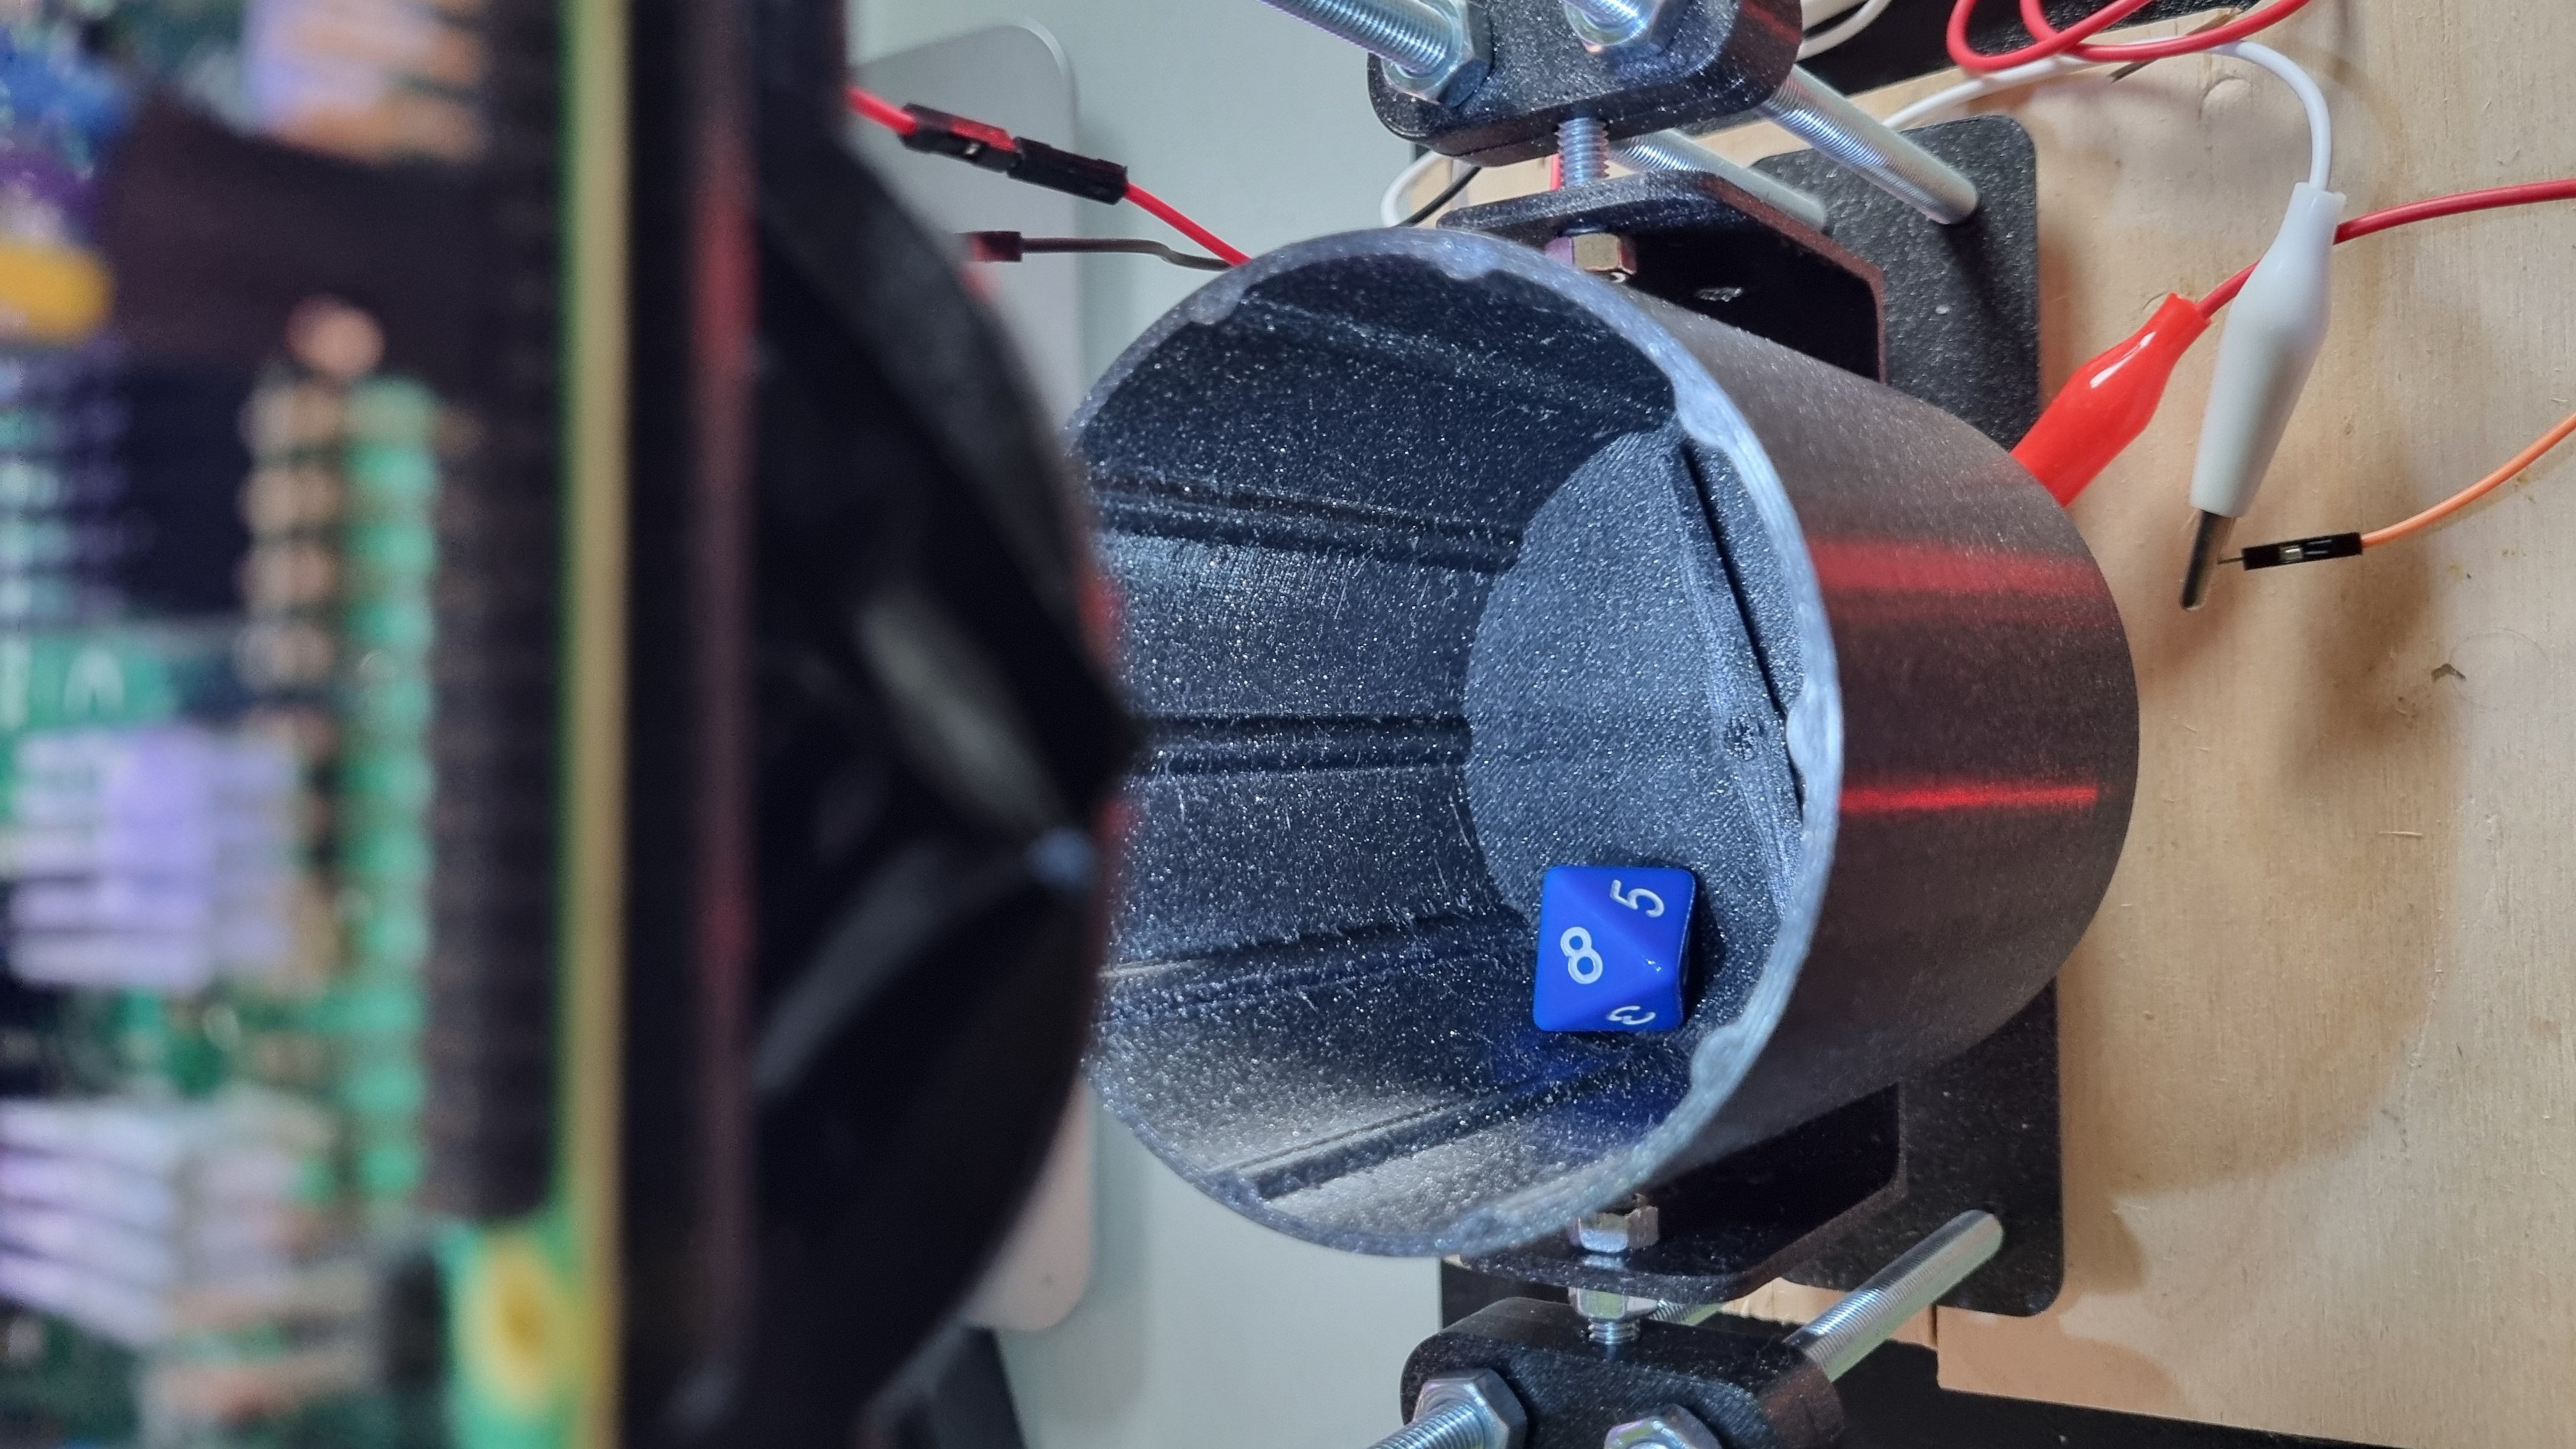
\includegraphics[width=0.45\linewidth]{chapters/03-praca-wlasna/figures/i_stala_sie_jasnosc.jpg}}
    \caption{\label{fig:jasno}Oświetlone wnętrze kubka}
\end{figure}

Po skonstruowaniu obu wersji robota oczywistym stało się, że wariant blendera będzie znacznie szybciej (około 4-krotnie) wykonywał rzut kością.
Pojedyńczy rzut kością wraz ze zrobieniem zdjęcia trwa około 1.7 sekundy.
Ponadto wersja blendera jest znacznie stabilniejszą konstrukcją, ponieważ nie wymaga poruszania dużymi komponentami robota. 
Największą zaletą wariantu blendera jest prostsza - w porównaniu z wariantem betoniarki - budowa spowodowana mniejszą liczbą ruchomych elementów. Jest to ważne z punktu widzenia
długotrwłej eksploatacji podczas, której bardziej skomplikowane mechanizmy szybciej się zużywają. Z tych powodów do docelowego robota wybrano 
wariant blendera. Dzięki temu projekt stał się mniej skomplikowany mechanicznie a jednocześnie jego użyteczność wzrosła, ponieważ
głównym zadaniem tego robota jest generowanie liczb losowych a to zadanie szybciej był w stanie wykonywać właśnie ten wariant.

\subsection{Ostateczna wersja robota}
Projektowanie ostatecznej wersji robota rozpoczęto od przeanalizowania wad, zalet oraz ogólnych cech (takich jak wymiary) prototypów.
Postanowiono, że finalna wersja robota będzie wykorzystywała kubek o tej samej średnicy co prototypowa. Dookoła tych wymiarów zaprojektowano 
resztę konstrukcji. Obudowę zaprojektowano w taki sposób żeby była w stanie pomieścić
kubek oraz kamerę umieszczoną na wysokości 120mm nad dnem kubka. Wysokość tą określono na podstawie jakości zdjęć jako najlepszą, podczas testów prototypów.
Dodatkowo w tylnej oraz dolnej części obudowy pozostawiono przestrzeń na resztę
elementów składowych robota. Rozmiar tej przestrzeni wyznaczono poprzez zwymiarowanie pozostałych elementów takich jak silnik, sterownik, wentylator 
czy Raspberry Pi. Te wymiary posłużyły do wyznaczenia minimalnej potrzebnej przestrzeni. To minimum zwiększono w taki sposób
żeby we wnętrzu pomieściły się również przewody i śruby oraz żeby po całkowitym złożeniu pozostała przestrzeń do swobodnego manipulowania
elementami składowymi.

Każdy element został zaprojektowany w taki sposób żeby cały robot był modułowy. Żeby spełnić to założenie, każdy element
zaprojektowano w taki sposób żeby posiadał on specjalne miejsca na inserty lub śruby. Inserty to mosiężne elementy, które za pomocą lutownicy wgrzewa się
w wydruk 3D. Posiadają one wewnętrzny gwint dzięki czemu można do łączenia wydruków wykorzystywać śruby nie uszkadzając samego wydruku przy 
wielokrotnym skręcaniu i rozkręcaniu robota. Dzięki temu założenie modułowości zostało spełnione, ponieważ dzięki śrubom i insertom każdy element robota 
mógł zostać wydrukowany jako osobna część, którą następnie połączono z innymi częściami w prosty do rozłożenia sposób.

\subsubsection{Opis komponentów ostatecznej wersji robota}

Górna część obudowy - pokrywa - mieszcząca kamerę oraz diody LED, została zaprojektowana w taki sposób żeby dostęp do kubka pozostał łatwy. Osiągnięto to
poprzez wykorzystanie prostego mocowania pokrywy do obudowy, z wykorzystaniem pojedyńczej śruby oraz magnesów neodymowych. Dzięki temu w przypadku kiedy konieczny 
jest dostęp do kamery lub diod LED wystarczy zdjąć tylną scianę robota oraz odkręcić pojedyńczą śrubę. Dodatkowo magnesy neodymowe zapewniają
dobre przyleganie pokrywy do reszty obudowy. Ich dodatkową zaletą jest blokowanie pokrywy w ustalonej pozycji podczas umieszczania kości wewnątrz
kubka.

\begin{figure}[H]
    \centering
    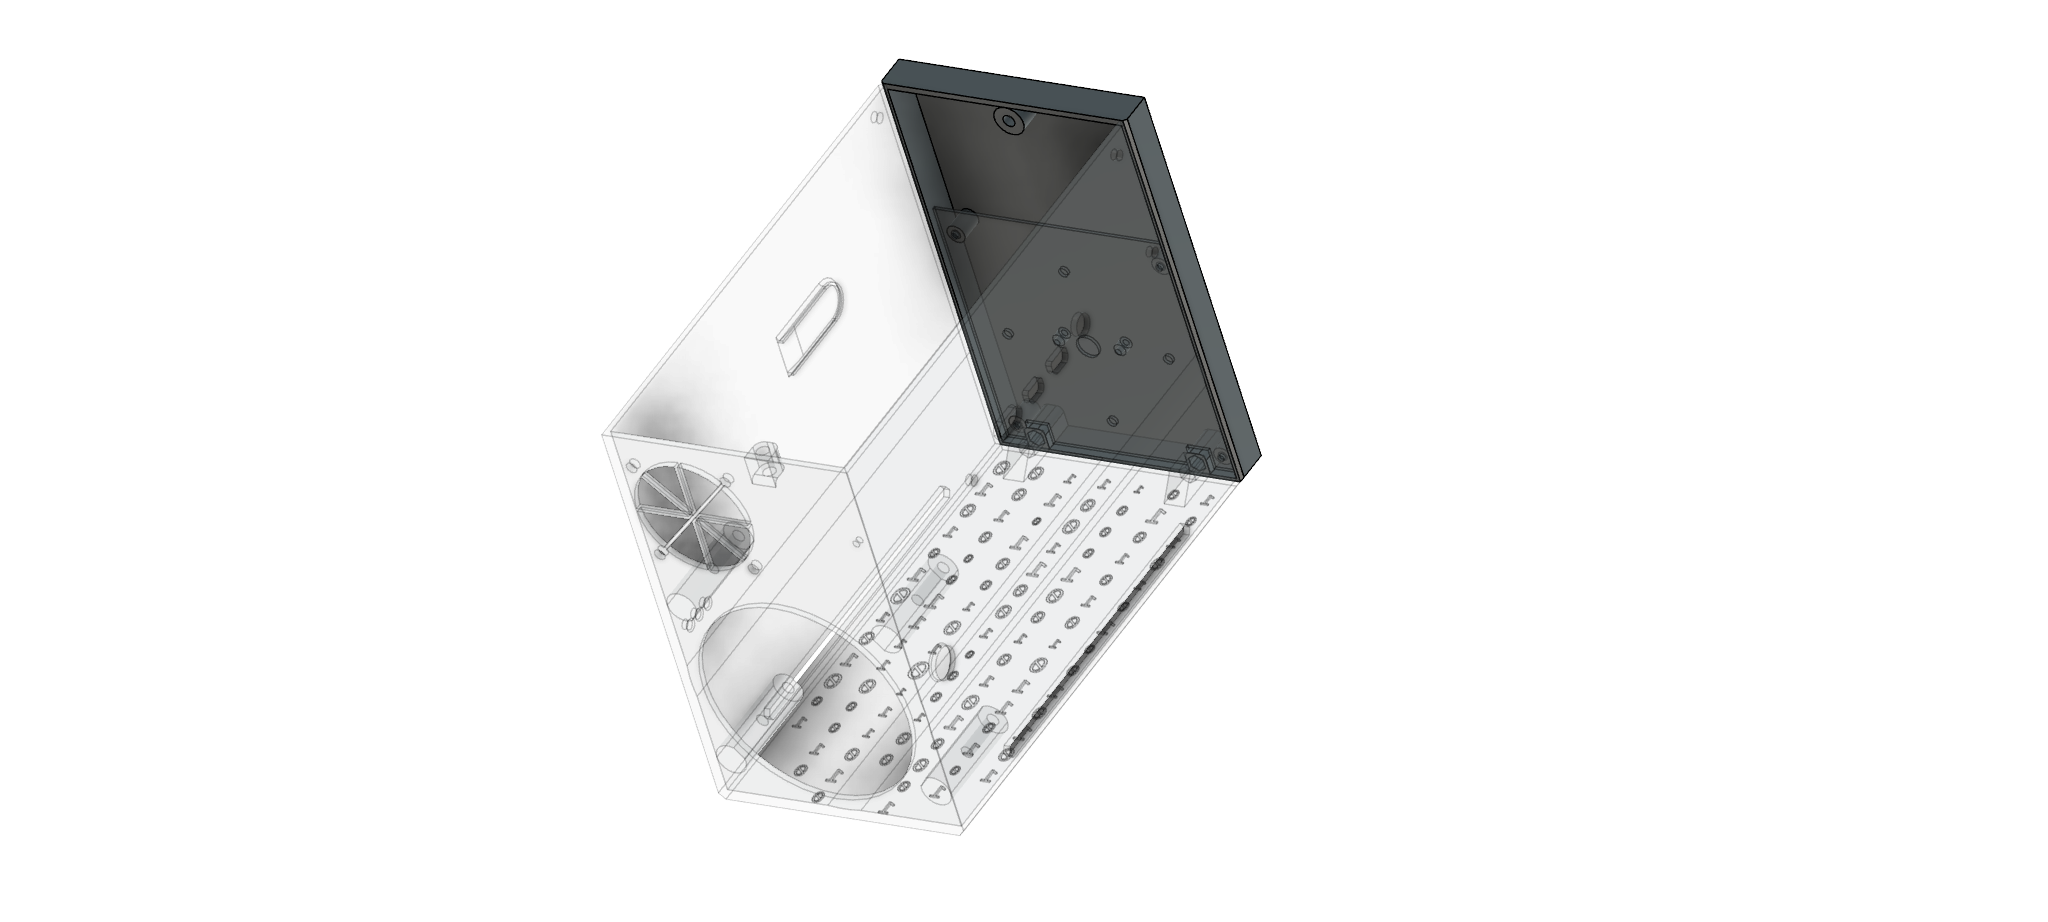
\includegraphics[width=0.95\linewidth]{chapters/03-praca-wlasna/figures/pokrywa.png}
    \caption{\label{fig:pokrywa}Pokrywa obudowy}
\end{figure}

Kamera wraz z diodami LED służącymi do oświetlenia wnętrza kubka znajdujde się w pokrywie. Kamerę zamontowano przy użyciu dwóch śrub M2 natomiast
diody LED umieszczono w zaprojektowanych w wydruku otworach.

W pokrywie znajdują się również dwa sześciokątne otwory na magnesy neodymowe. Dzięki temu że otwory są sześciokątne to walcowe magnesy idealnie
się w nie wpasowują i po wciśnięciu nie wypadają. W drugiej części obudowy znajdują się takie same otwory na drugą parę magnesów. Dla pewności podczas umieszczania magnesów 
wykorzystano klej cyjanoakrylowy.

Kubek, w którym dokonywane są rzuty kością, zaprojektowano na podstawie kubka z prototypowej wersji blendera. Zachowano jego średnicę oraz kształt i rozmieszczenie wewnętrznych
żeber. Zmieniona została zasada mocowania kubka w taki sposób, żeby był on przystosowany do zamocowania w obudowie. W tym celu zaprojektowano
cztery mocowania, znajdujące się u dołu kubka, za pomocą których kubek jest przykręcany do obudowy. Dodatkowo pogrubiono dno kubka tak żeby można było w nim umieścić inserty służące 
do przykręcenia uchwytu silnika. Ostatnią modyfikacją było podwyższenie kubka w taki sposób, żeby wysokością sięgał on aż do mocowania kamery - górnej pokrywy.
Dzięki temu podczas rzutów zniknął problem z wypadającą kością co było dość częstym zajwiskiem podczas testów prototypu. Niestety takie rozwiązanie
spowodowało, że wnętrze kubka przestało być widoczne z zewnątrz. Jednak zostało uznane, że widok z zewnątrz na wnętrze kubka nie jest konieczny do osiągnięcia celów projektu.

\begin{figure}[H]
    \centering
    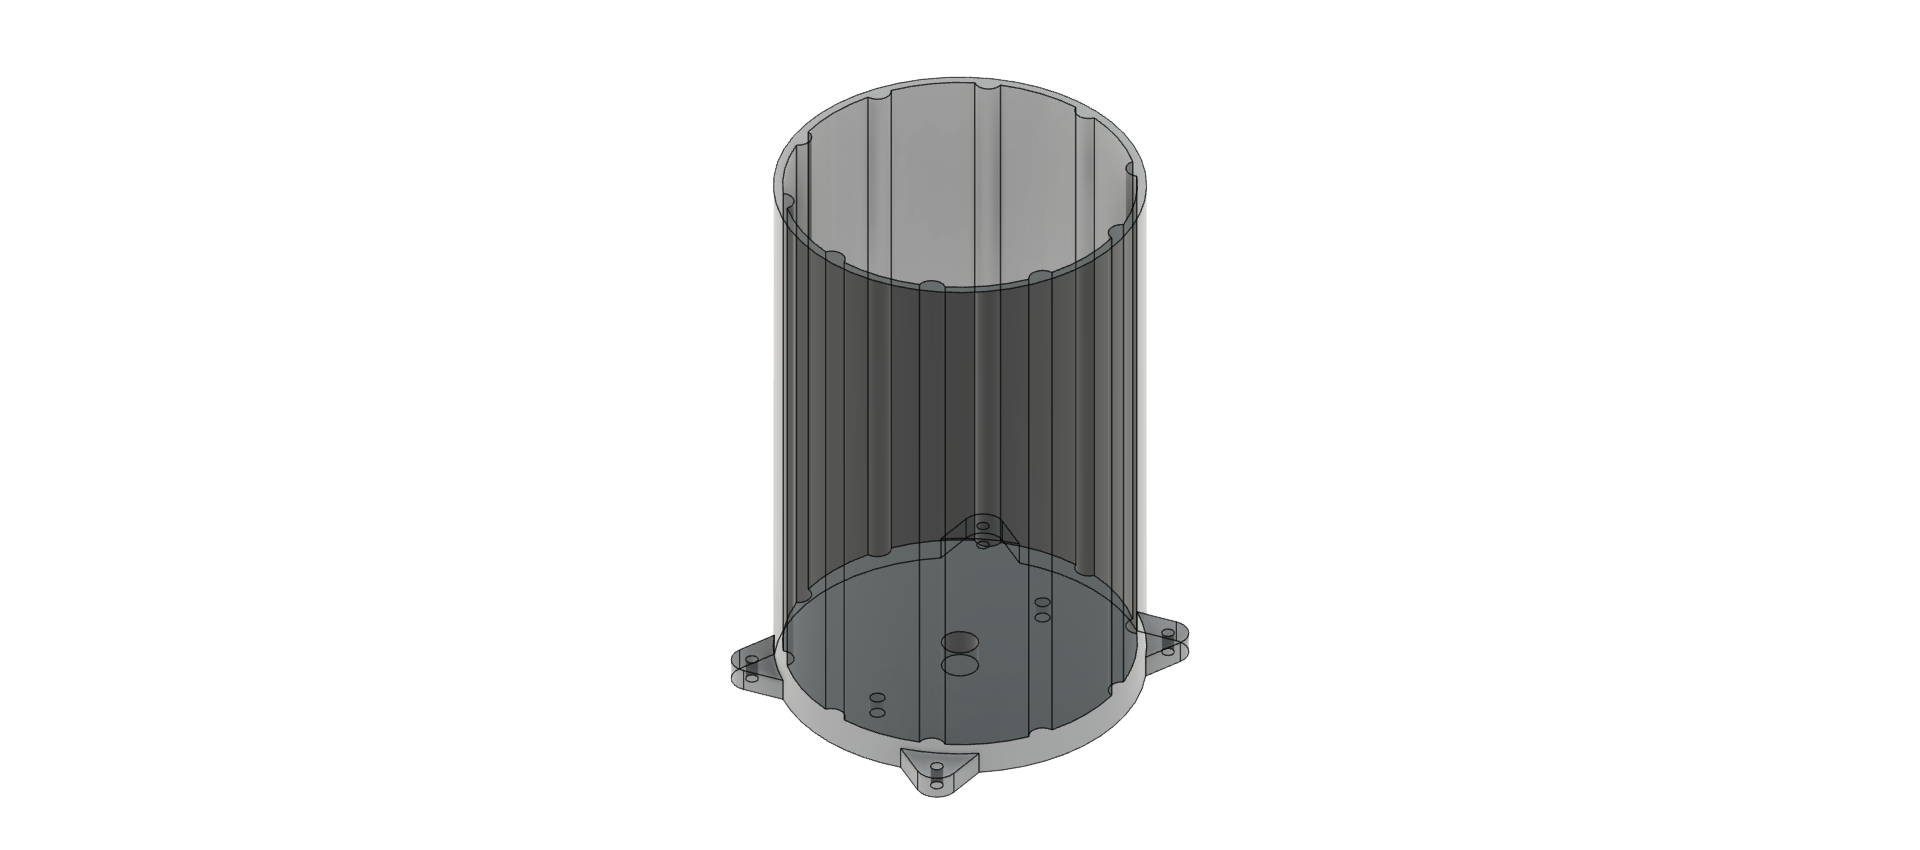
\includegraphics[width=0.95\linewidth]{chapters/03-praca-wlasna/figures/kubek.png}
    \caption{\label{fig:kubek}Kubek}
\end{figure}

Projekt pierwszego uchwytu mocującego silnik składał się z miejsca do umieszczenia silnika oraz dwóch cylindrycznych słupków służących za prowadnice
śrub mocujących cały uchwyt do dna kubka. Jednak, ponieważ podczas testów pojawiły się problemy z pierwszym silnikiem i wymieniono go na inny, konieczne
było zaprojektowanie drugiego uchwytu. Podczas projektowania drugiego uchwytu wzorowano sie na projekcie pierwszego, jednak dodano dodatkowy trzeci
cylindryczny słupek na śrubę, która miała służyć do kontrolowania wychylenia całego uchwytu w osi przód-tył. Zwiększyło to możliwość regulacji i w ten sposób
ograniczono tarcie śmigla o dno kubka. 

Śmigło zaprojektowano w taki sposób żeby obracając się przy samym dnie kubka, po uderzeniu w kość, wybijało ją w górę. Ten efekt uzyskano
dzięki niskiemu profilowi śmigła oraz bocznych ścian śmigła nachylonych pod kątem $45^{\circ}$.

Podczas testów ostatecznej wersji robota napotkano wcześniej wspominane problemy z pierwotnie wykorzystywanym silnikiem. Silnik ten miał okrągły wał przez co śmigło musiało
być bardzo dokładnie spasowane aby uniknąć ślizgania się wału wewnątrz otworu śmigła. To sprawiało, że montowanie śmigła i jego demontaż był bardzo trudny. Dodatkowo po wielokrotnych rzutach kością, śmigło
wbijało się coraz niżej na wał silnika i w ostateczności tarło o dno kubka tak mocno, że silnik nie był w stanie się obracać. 
Żeby temu zaradzić umieszczono pomiędzy śmigłem a dnem kubka metalową podkłądkę, po której śmigło mogło się ślizgać łatwiej niż po dnie kubka. To
jednak nie rozwiązało problemu ponieważ po kolejnych kilku tysiącach rzutów śmigło zaczęło się blokować. 
Z tego powodu postanowiono wymienić silnik na mocniejszy 12V silnik z przekładnią, który ma mniejszą częstotliowść obrotu (około 1000RPM zamiast 4000RPM) ale ma większy moment obrotowy.
Zaletą nowego silnika jest jego wał w kształcie litery "D". Pozwala to na znacznie luźniejsze spasowanie otworu śmigła z wałem przez co 
demontaż śmigła jest znacznie łatwiejszy. Ponadto nowy silnik jest znacznie cichszy niż poprzedni .

\begin{figure}[H]
    \centering
    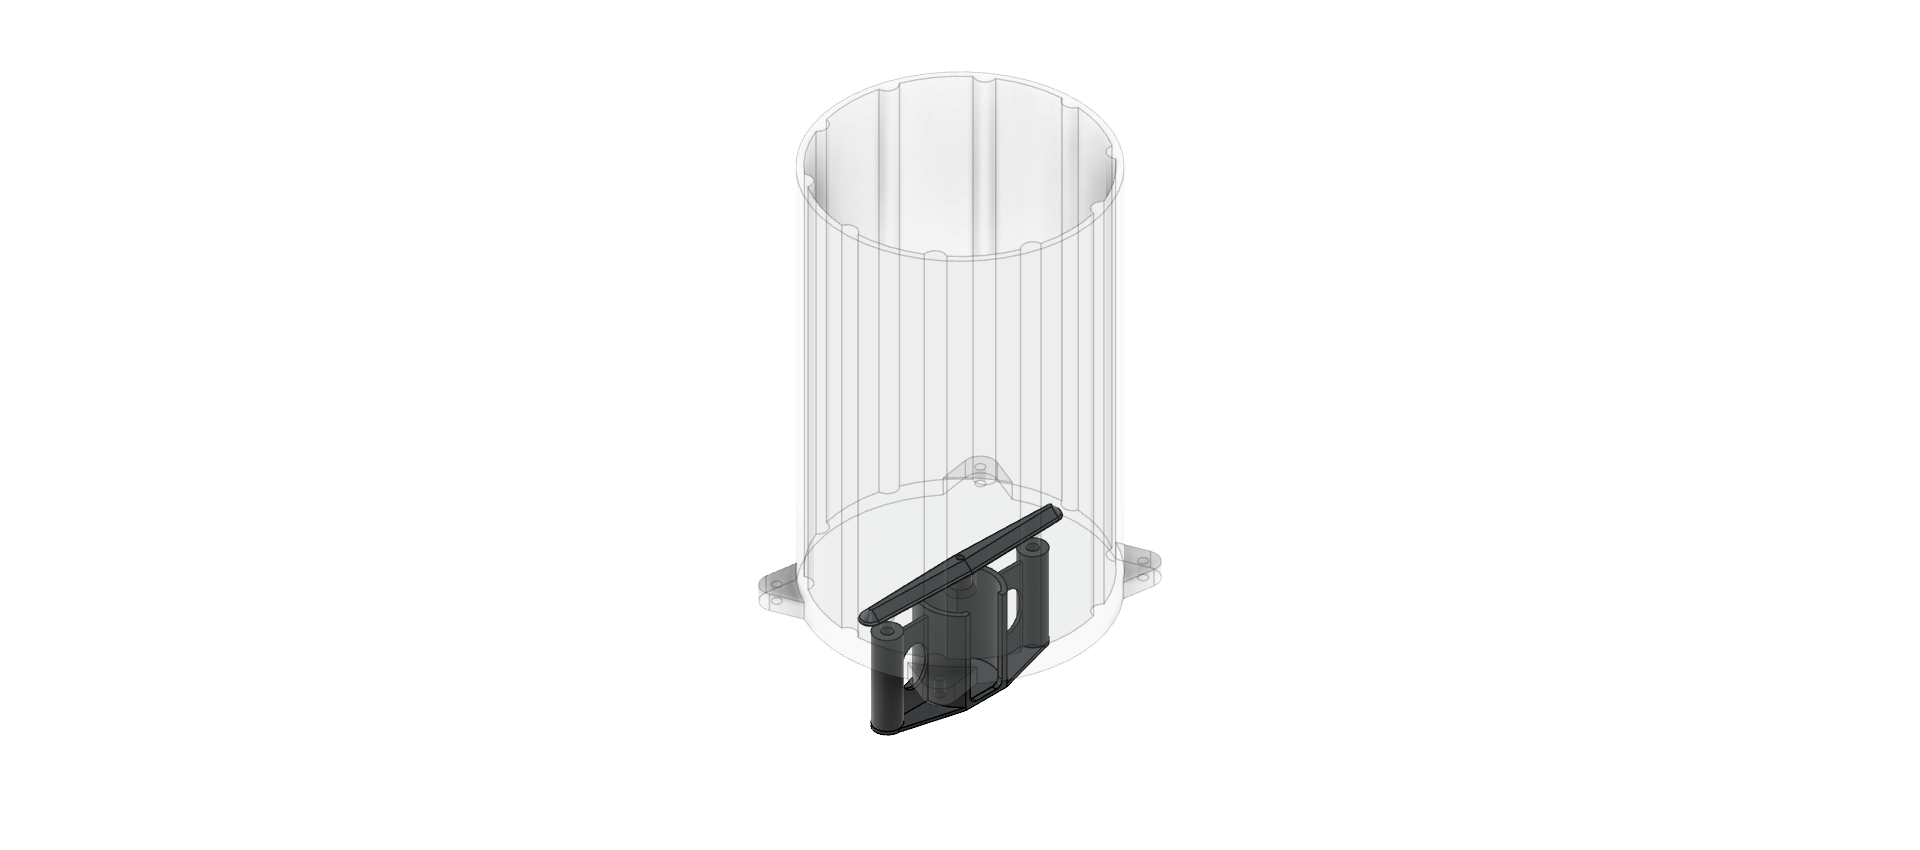
\includegraphics[width=0.95\linewidth]{chapters/03-praca-wlasna/figures/uchwyt_v1.png}
    \caption{\label{fig:uchwyt_v1}Pierwsza wersja uchwytu silnika oraz śmigło względem kubka}
\end{figure}

\begin{figure}[H]
    \centering
    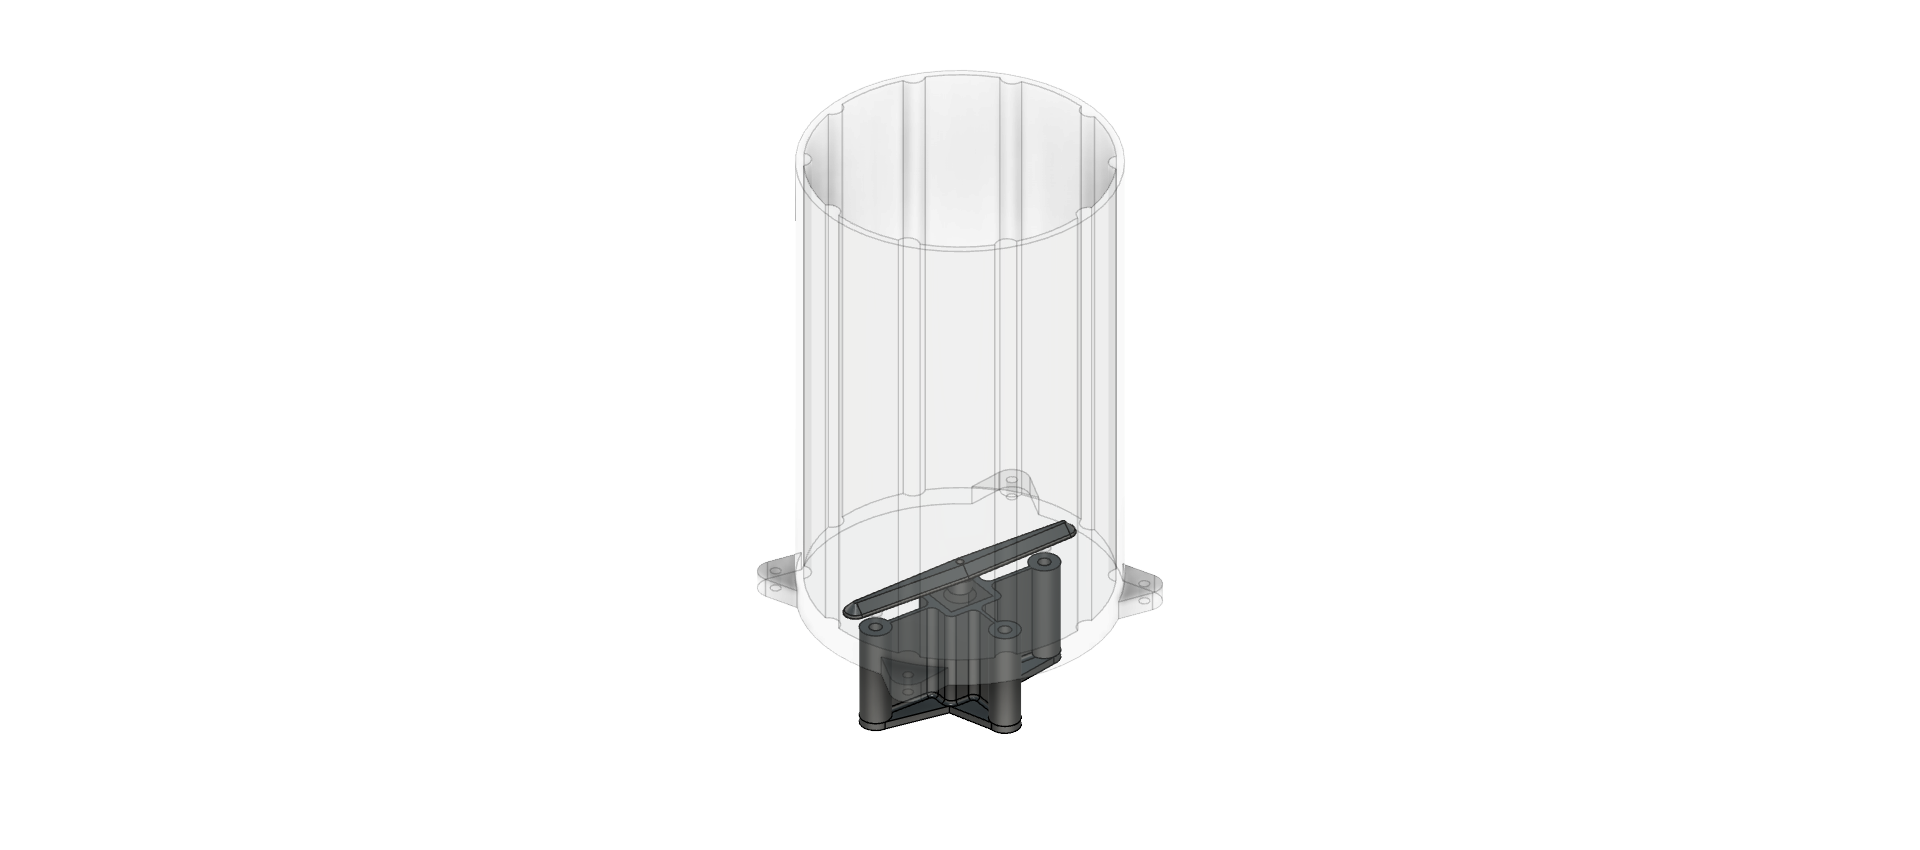
\includegraphics[width=0.95\linewidth]{chapters/03-praca-wlasna/figures/uchwyt_v2.png}
    \caption{\label{fig:uchwyt}Druga wersja uchwytu silnika oraz śmigło względem kubka}
\end{figure}

Do mocowania Raspberry Pi zaprojektowano specjalną płykę przykręcaną do boku obudowy. W projekcie tej płytki uwzględniono otwory do przymocowania Raspberry
Pi oraz układu ULN2803A Darlington. Dodatkowo przygotowano specjalne miejsce do mocowania przycisku. Na płytnce pozostawiono również miejsce
na zamontowanie szyny zasilania. Płytkę tą umieszczono w obudowie w taki sposób, żeby znajdowała się ona bezpośrednio nad wentylatorem. Dzięki temu
strumień powietrza bezpośrednio chłodzi najważniejsze elementy elektroniczne robota. Przycisk zamocowano na tej samej płytce, z wykorzystaniem
dodatkowego elementu wydukowanego na drukarce 3D. Dzięki temu znalazł się on bezpośrednio przy ściance obudowy, a dodatkowo jego mocowanie
nadal spełnia założenie modułowości poprzez mocowanie za pomocą śrub i insertów.

\begin{figure}[H]
    \centering
    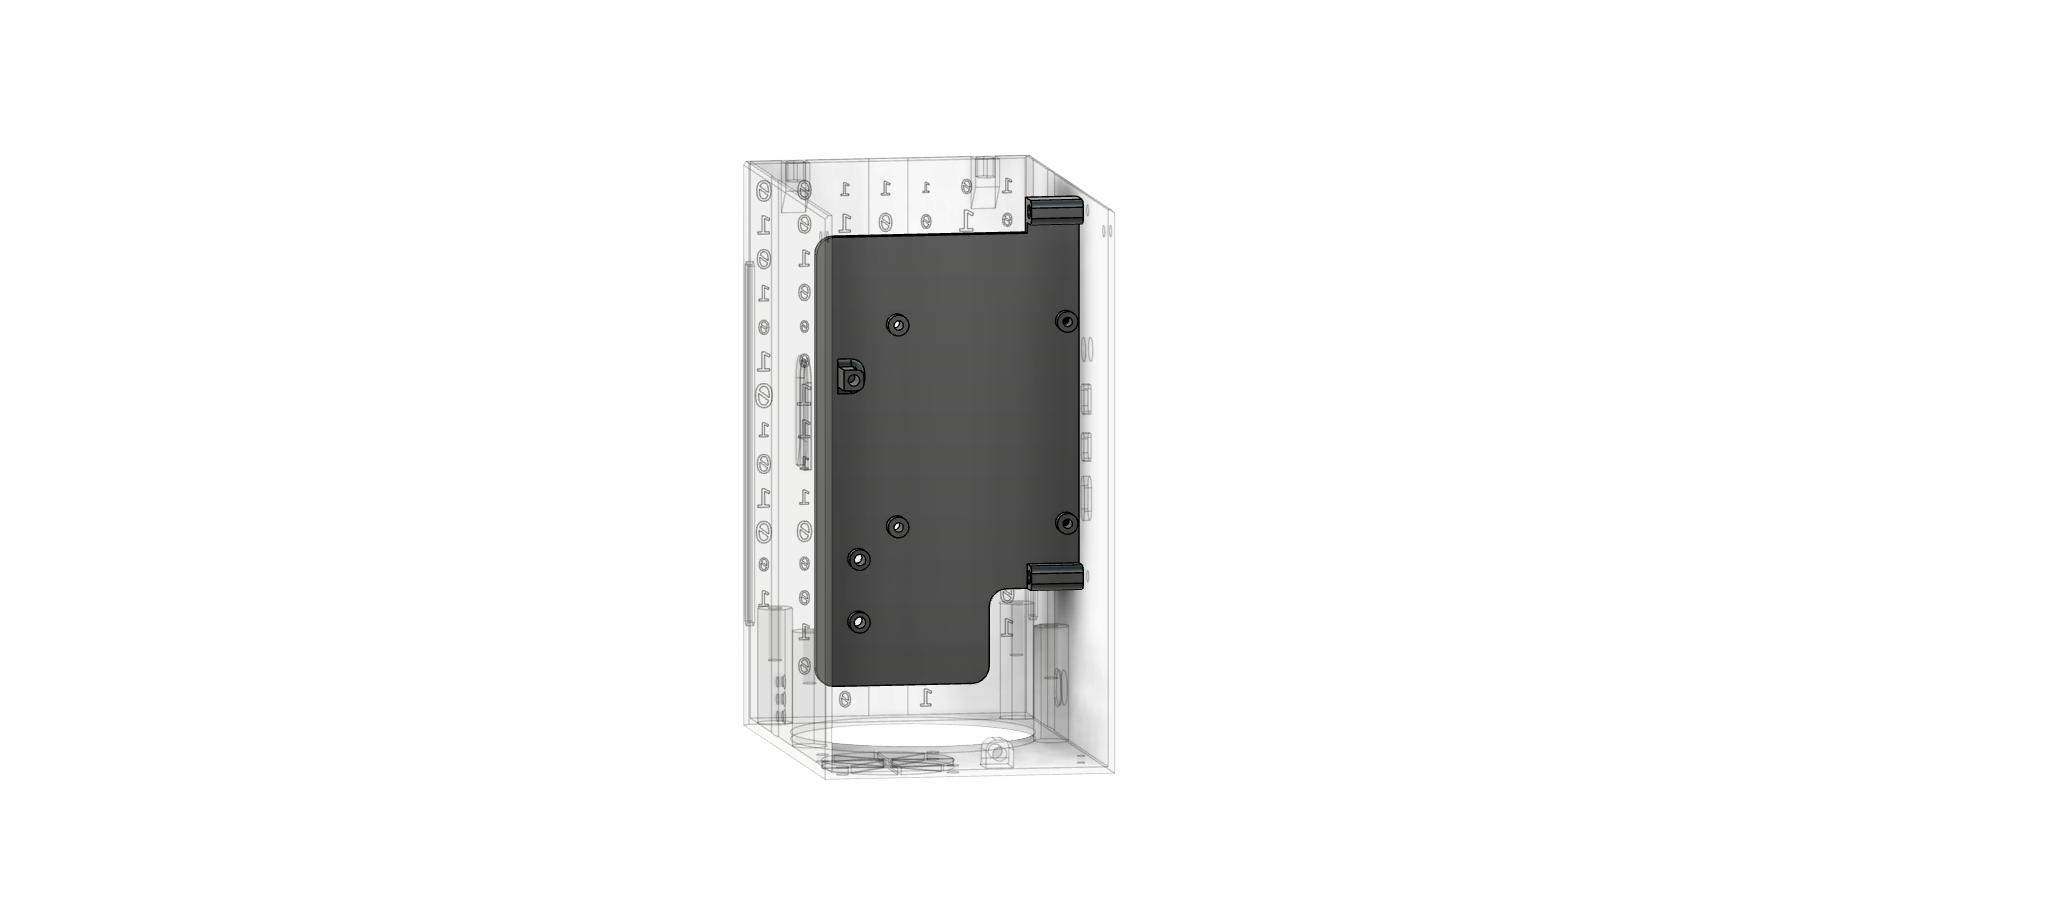
\includegraphics[width=0.95\linewidth]{chapters/03-praca-wlasna/figures/main_board.png}
    \caption{\label{fig:mainboard}Płytka do montażu elektroniki}
\end{figure}

Układ sterujący silnikiem L298 przykręcono do obudowy pośrednio, poprzez specjalnie zaprojektowane i wydrukowane mocowanie. Dzięki temu wykorzystano
gotowe otwory na śruby znajdujące się w płytce układu L298.

Do dna obudowy robota przymocowano za pomocą śrub również wentylator.

\begin{figure}[H]
    \centering
    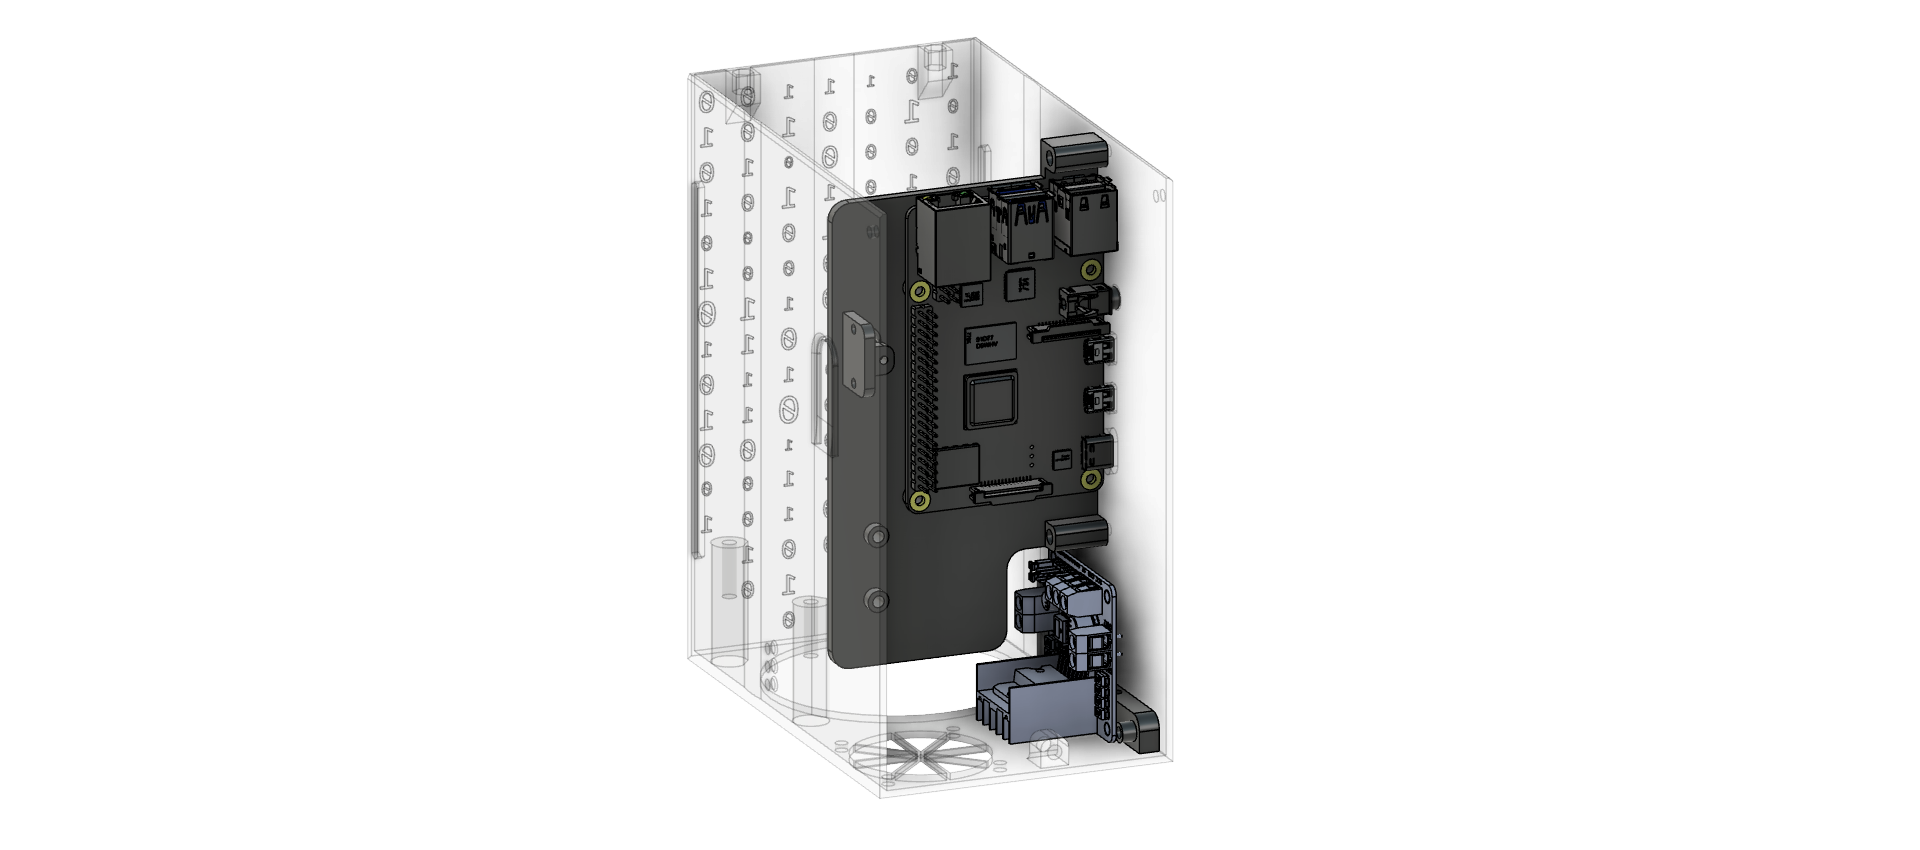
\includegraphics[width=0.95\linewidth]{chapters/03-praca-wlasna/figures/l298n.png}
    \caption{\label{fig:steownik}Zamocowany sterownik L298 z widoczną płytką na której zamocowana jest Raspberry Pi 4b}
\end{figure}

Obudowę zaprojektowano w taki sposób żeby pomieściła wszystkie powyższe elementy. W jej scianach zaprojektowano otwory na wyjścia Raspberry Pi, 
diody LED oraz gniazdo zasilania. W scianie obudowy na wysokości miejsca, w którym znajduje się wewnątrz przycisk, zaprojektowano specjalne wycięcie.
Dzięki dodatkowemu zmniejszeniu grubosci sciana obudowy w tym miejscu jest bardziej elastyczna co pozwala na kliknięcie przycisku znajdującego
się po wewnętrznej stronie ściany obudowy. Na dnie obudowy zaprojektowo również specjalne słupki służące za podpórki dla kubka. 
W słupkach tych zaprojektowano otwory na inserty dzięki, którym kubek można przykręcić do obudowy gwarantując tym jego stabilność.

Podczas projektowania obudowy przewidziano także takie elemementy jak wycięcia od spodu bezpośrednio pod wentylatorem, służące za wlot powietrza 
oraz wycięcia w tylnej ściance, służące za wylot powietrza. Dodatkowo w dnie umieszczono duży utwór możliwiający swobodne mocowanie oraz dostęp do 
silnika, diod LED oraz gniazda zasilania. Na bocznych ścianach zaprojektowano przerwy, które następnie zaślepiono kontrastującym kolorystycznie filamentem.
Przerwy te tak samo jak cyfry na przedniej ścianie obudowy są tylko i wyłącznie elemetami estetycznymi. Ostatnim elementem robota są zaprojektowane nóżki, 
które przyklejono do dna robota. Zapewniają one przepływ powietrza pod robotem gdzie znajduje się wlot powietrza do wentylatora.

\begin{figure}[H]
    \centering
    \includegraphics[width=0.95\linewidth]{chapters/03-praca-wlasna/figures/całosc_front.png}
    \caption{\label{fig:gotowy}Projekt gotowego robota od frontu}
\end{figure}